% Compilation : pdflatex Cinematique_des_fluides.tex (deux fois).
% Texte, equations et figures TikZ modifiables ; aucun fichier externe requis.
% Les commentaires « Source » reperent les pages du manuscrit.
\documentclass[11pt,a4paper]{article}
\usepackage[utf8]{inputenc}
\usepackage[T1]{fontenc}
\usepackage[provide=*,french]{babel}
\usepackage[scaled=0.95]{helvet}
\renewcommand{\familydefault}{\sfdefault}
\usepackage{amsmath,amssymb,esint}
\usepackage{geometry}
\geometry{left=15mm,right=15mm,top=18mm,bottom=18mm,headheight=14pt,headsep=6mm}
\usepackage{fancyhdr,lastpage}
\usepackage{tikz}
\usetikzlibrary{arrows.meta,calc,decorations.pathreplacing,decorations.markings,angles,quotes}
\usepackage[most]{tcolorbox}
\usepackage{enumitem}
\usepackage{titlesec}
\usepackage{needspace}
\usepackage{hyperref}
\hypersetup{hidelinks,pdftitle={Cinématique des fluides},pdfsubject={Cours de physique}}
\pagestyle{fancy}\fancyhf{}
\fancyhead[L]{\small Physique F2 - Cinématique des fluides - inspiré par les cours de Mme Mesnil}
\fancyhead[R]{\small\thepage/\pageref{LastPage}}
\fancyfoot[R]{\small PC-PC*}
\renewcommand{\headrulewidth}{0pt}
\setlength{\parindent}{0pt}
\setlength{\parskip}{5pt}
\setlength{\abovedisplayskip}{8pt}
\setlength{\belowdisplayskip}{8pt}
\setlist[itemize]{leftmargin=5mm,itemsep=3pt,topsep=3pt,label=\(\rightarrow\)}
\titleformat{\section}{\Large\bfseries}{\Roman{section}.}{0.4em}{}
\titleformat{\subsection}{\large\bfseries}{\Roman{section}.\arabic{subsection}.}{0.4em}{}[\titlerule]
\titlespacing*{\section}{0pt}{11pt}{5pt}
\titlespacing*{\subsection}{0pt}{9pt}{5pt}
\newtcolorbox{cadre}[1][]{enhanced,sharp corners,colback=white,colframe=black,boxrule=1.1pt,left=7pt,right=7pt,top=5pt,bottom=5pt,before skip=7pt,after skip=7pt,#1}
% Les étoiles sont placées à droite, en dehors du cadre.
\tcbset{etoiles/.style={width=\dimexpr\linewidth-22mm\relax,
  overlay={\node[anchor=west,inner sep=0pt,font=\small]
    at ([xshift=2mm]frame.east) {\(#1\)};}}}
\newcommand{\dd}{\mathrm d}
\newcommand{\vv}{\vec v}
\newcommand{\JJ}{\vec{j}}
\newcommand{\OO}{\vec\Omega}
\newcommand{\OM}{\overrightarrow{OM}}
\newcommand{\grad}{\overrightarrow{\mathrm{grad}}}
\newcommand{\rot}{\overrightarrow{\mathrm{rot}}}
\newcommand{\ddiv}{\operatorname{div}}
\newcommand{\Dt}[1]{\frac{\mathrm D #1}{\mathrm D t}}
\newcommand{\pd}[2]{\frac{\partial #1}{\partial #2}}
\newcommand{\etoiles}[1]{\hfill\(\underbrace{\vphantom{A}#1}_{\vphantom{A}}\)}
\newcommand{\rem}{\underline{Remarques :}\ }
\tikzset{>=Stealth,every node/.style={font=\small},flow/.style={thick,->},edge/.style={thick},old/.style={thick,dashed},new/.style={very thick}}
% Schéma d'une particule suivie entre deux instants.
\newcommand{\particule}[1]{%
\begin{tikzpicture}[scale=.9]
\draw (0,0) ellipse (.15 and .19);\node[left] at (-.1,.1){$M(t)$};\node[below] at (0,-.2){$\dd^3\tau$};
\draw[flow] (0,0)--(1.4,.65) node[midway,above left]{\ifnum#1=0 $\vv(M,t)$\else $\vv(\OM,t)$\fi};
\draw[dashed] (1.4,.65)--(2.3,1.1);\draw (2.3,1.1) ellipse (.15 and .19);
\node[above] at (2.3,1.3){$M(t+\dd t)$};
\ifnum#1=1 \draw[flow] (2.3,1.1)--(3.7,1.45) node[right]{$\vv(\OM+\dd\OM,t+\dd t)$};\fi
\end{tikzpicture}}
% Lignes de courant courbes.
\newcommand{\courant}[1]{%
\begin{tikzpicture}[scale=.66]
\draw[edge] (0,1.5) .. controls (1.8,3.0) and (3.4,3.5) .. (5,3.9);
\draw[edge] (0,-1.1) .. controls (1.8,.4) and (3.4,.9) .. (5,1.3);
\foreach \a in {-.5,.2,.9}{\draw[flow] (0,\a) .. controls (1.8,1.5+\a) and (3.4,2+\a) .. (4.7,2.35+\a);}
\node[below left] at (1.9,1.47){$M$};
\draw (1.8,1.4)--(2,1.6);\draw (1.8,1.6)--(2,1.4);
\ifnum#1=1
\draw[dashed] (1.9,1.5)..controls (2.3,1.75)..(2.7,1.96);
\draw (2.6,1.86)--(2.8,2.06);\draw (2.6,2.06)--(2.8,1.86);
\node[right,align=left] at (5.5,1.4){La ligne de champ de vitesse\\coïncide avec la trajectoire.};
\else \draw[flow] (1.9,1.5)--(2.7,1.96);\fi
\end{tikzpicture}}
% Normales calculées à partir de la tangente locale du tracé.
\tikzset{normale/.style args={#1/#2}{postaction={decorate},
 decoration={markings,mark=at position #1 with{\draw[flow] (0,0)--(0,#2);}}}}
% Surface quelconque orientée.
\newcommand{\surface}[2]{%
\begin{tikzpicture}[scale=.7]
\draw[edge] (0,0) .. controls (-.8,.7) and (.3,1.7) .. (-.1,2.3) .. controls (-.4,3.2) and (.4,3.5) .. (.8,3) .. controls (2.7,3.5) and (2.3,2.5) .. (1.6,1.8) .. controls (1.1,.8) and (1.7,.2) .. (.7,-.2) .. controls (.3,-.4) and (.1,-.1) .. (0,0);
\node[above] at (1,3.2){$#1$};
\path[postaction={decorate},decoration={markings,
 mark=at position .5 with{\draw[flow] (0,0)--(0,1.05) node[above,transform shape=false]{$\vec n$};}}]
 (1.6,1.8) .. controls (1.1,.8) and (1.7,.2) .. (.7,-.2);
\ifnum#2=1
\path[normale=.45/.9] (.8,3) .. controls (2.7,3.5) and (2.3,2.5) .. (1.6,1.8);
\path[normale=.85/.9] (1.6,1.8) .. controls (1.1,.8) and (1.7,.2) .. (.7,-.2);
\fi
\end{tikzpicture}}
% Tube de champ (normales sortantes ou débits orientés).
\newcommand{\tube}[1]{%
\begin{tikzpicture}[scale=.8]
\draw[edge] (0,0) ellipse (.15 and .35);\draw[edge] (4,0) ellipse (.45 and 1.25);
\draw[edge] (0,.35)..controls (1.7,.5) and (2.8,.8)..(4,1.25);
\draw[edge] (0,-.35)..controls (1.7,-.5) and (2.8,-.8)..(4,-1.25);
\node[above] at (0,.45){$S_1$};\node[above] at (4,1.3){$S_2$};
\ifnum#1=1
\draw[flow] (0,0)--(-.8,0);\draw[flow] (4,0)--(5,0);
\path[postaction={decorate},decoration={markings,mark=at position .25 with{\draw[flow] (0,0)--(0,.75);},mark=at position .68 with{\draw[flow] (0,0)--(0,.75);}}] (0,.35)..controls (1.7,.5) and (2.8,.8)..(4,1.25);
\path[postaction={decorate},decoration={markings,mark=at position .25 with{\draw[flow] (0,0)--(0,-.75);},mark=at position .68 with{\draw[flow] (0,0)--(0,-.75);}}] (0,-.35)..controls (1.7,-.5) and (2.8,-.8)..(4,-1.25);
\draw[flow] (.7,.38)--(1.5,.49);\draw[flow] (.7,-.38)--(1.5,-.49);
\node at (2,1.25){$S_L$};\node at (2,-1.25){$S_L$};
\node[right,align=left] at (5,.7){Tube de champ de $\vv$};
\node[below] at (2,-1.6){La surface fermée est orientée vers l'extérieur.};
\else
\draw[flow] (-.4,-.13)--(.7,-.13);\draw[flow] (-.4,.13)--(.7,.13);
\foreach \y in {-.7,0,.7}{\draw[flow] (4,\y)--(5.2,\y);}
\node[below] at (0,-.6){$D_{v1}$};\node[below] at (4,-1.4){$D_{v2}$};
\fi
\end{tikzpicture}}
% Déformation des exemples a), b), c) : tous les tracés sont éditables.
\newcommand{\deformation}[1]{%
\begin{tikzpicture}[scale=.83]
\draw[->] (0,0)--(6,0) node[right]{$x$};\draw[->] (0,0)--(0,4.2) node[above]{$y$};
\node[below left] at (0,0){$O$};\draw[old] (0,0) rectangle (3,3);
\node[above] at (1.4,3.5){$t$};\node at (4.8,2){$t+\dd t$};
\draw[<->] (0,-.7)--(3,-.7) node[midway,below]{$L$};
\draw[<->] (-1.05,0)--(-1.05,3) node[midway,left]{$L$};
\ifnum#1=1
\draw[new] (0,0) rectangle (3.8,2.25);
\draw[flow] (3,0)--(3.8,0) node[midway,below=2pt]{$a_1L\dd t$};
\draw[flow] (0,3)--(0,2.25) node[midway,right]{$b_1L\dd t$};
\draw[dashed] (3,3)--(3.8,3)--(3.8,2.25);
\draw[flow] (3,3)--(3.8,2.25);\node[above] at (3.4,3){$a_1L\dd t$};\node[right] at (3.8,2.6){$b_1L\dd t$};
\fi
\ifnum#1=2
\draw[new] (0,0)--(3,.75)--(3.75,3.75)--(.75,3)--cycle;
\draw[flow] (0,3)--(.75,3) node[midway,above]{$a_2L\dd t$};
\draw[flow] (3,0)--(3,.75) node[midway,right]{$a_2L\dd t$};
\draw[dashed] (3,3)--(3.75,3)--(3.75,3.75);
\draw[flow] (3,3)--(3.75,3.75);\node[below] at (3.4,3){$a_2L\dd t$};\node[right] at (3.75,3.4){$a_2L\dd t$};
\fi
\ifnum#1=3
\draw[new] (0,0)--(3,.75)--(2.25,3.75)--(-.75,3)--cycle;
\draw[flow] (0,3)--(-.75,3) node[midway,above]{$a_3L\dd t$};
\draw[flow] (3,0)--(3,.75) node[midway,right]{$a_3L\dd t$};
\draw[dashed] (3,3)--(3,3.75)--(2.25,3.75);
\draw[flow] (3,3)--(2.25,3.75);\node[above] at (2.6,3.75){$a_3L\dd t$};\node[right] at (3,3.4){$a_3L\dd t$};
\draw[->] (1.4,0) arc (0:14:1.4);\node[right] at (1.4,.2){$\dd\theta$};
\fi
\end{tikzpicture}}
\begin{document}
% Source : pages 1-2.
{\fontsize{27}{31}\selectfont\bfseries Cinématique des fluides\par}
% Sommaire ajouté ; les titres reprennent ceux du cours.
\begingroup
\setlength{\parskip}{2pt}
\smallskip
\textbf{Introduction}\par
\medskip\textbf{I- Notion de dérivée particulaire}\par
\hspace*{10mm}\textit{1) Dérivée particulaire d'un champ scalaire}\par
\hspace*{10mm}\textit{2) Dérivée particulaire du champ des vitesses}\par
\medskip\textbf{II- Conservation de la masse}\par
\hspace*{10mm}\textit{1) Vecteur densité de courant de masse}\par
\hspace*{10mm}\textit{2) Débit massique}\par
\hspace*{10mm}\textit{3) Équation globale de conservation de la masse}\par
\hspace*{10mm}\textit{4) Équation locale de conservation de la masse}\par
\medskip\textbf{III- Écoulement stationnaire}\par
\hspace*{10mm}\textit{1) Propriétés du vecteur densité de courant de masse}\par
\hspace*{10mm}\textit{2) Conséquence sur le débit massique}\par
\medskip\textbf{IV- Écoulement incompressible}\par
\hspace*{10mm}\textit{1) Débit volumique}\par
\hspace*{10mm}\textit{2) Définition}\par
\hspace*{10mm}\textit{3) Propriété du champ des vitesses}\par
\medskip\textbf{V- Vecteur tourbillon - Dilatation d'une particule}\par
\hspace*{10mm}\textit{1) Problématique mathématique}\par
\hspace*{10mm}\textit{2) Quelques exemples}\par
\hspace*{10mm}\textit{3) Généralisation}\par
\hspace*{10mm}\textit{4) Cas de l'écoulement irrotationnel}\par
\hspace*{10mm}\textit{5) Cas de l'écoulement irrotationnel et incompressible}\par
\endgroup

\vspace{5mm}
{\Large\bfseries Introduction\par}
\medskip
\underline{Pour un solide}
\begin{center}
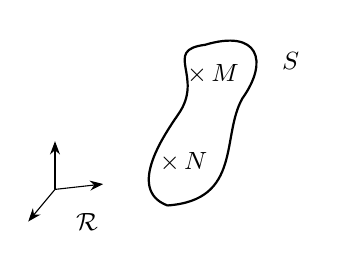
\begin{tikzpicture}[scale=.68]
\draw[edge] (1.6,0)..controls (.8,.3) and (1.6,1.4)..(1.8,1.7)..controls (2.3,2.4) and (1.5,2.9)..(2.3,3)..controls (3.3,3.3) and (3.5,2.7)..(3,2)..controls (2.6,1.3) and (3,.1)..(1.6,0);
\node at (2.45,2.45){$\times\,M$};\node at (1.9,.8){$\times\,N$};\node at (3.9,2.7){$S$};
\draw[->] (-.5,.3)--(-.5,1.2);\draw[->] (-.5,.3)--(.4,.4);\draw[->] (-.5,.3)--(-1,-.3);\node at (.1,-.3){$\mathcal R$};
\end{tikzpicture}
\end{center}
\[
\left(\frac{\dd\overrightarrow{MN}}{\dd t}\right)_{\mathcal R}
=\OO_{S/\mathcal R}\wedge\overrightarrow{MN}
\quad\Longleftrightarrow\quad
\vv_{\mathcal R}(M)=\vv_{\mathcal R}(N)+\OO_{S/\mathcal R}\wedge\overrightarrow{NM}.
\]
\(\rightarrow\) La vitesse d'un point du solide caractérise la vitesse du solide.

Un \underline{fluide} est un système déformable ; sa description est donc plus complexe.
\section{Notion de dérivée particulaire}
\subsection{Dérivée particulaire d'un champ scalaire}
\begin{center}\particule{0}\end{center}
On considère un champ scalaire $g(M,t)$ (par exemple, la température, la pression ou la masse volumique).\\
On cherche à exprimer la variation suivante :
\[
g\bigl(\underbrace{\OM+\vv(M,t)\dd t}_{\text{on suit la particule}},t+\dd t\bigr)-g(\OM,t),
\qquad \dd\OM=\vv(M,t)\dd t.
\]
\begin{cadre}
On note $\Dt{g}$ la \textbf{dérivée particulaire de $g$}.

Elle est définie comme la limite, quand $\dd t\to0$, du taux d'accroissement de $g$ mesuré en suivant la particule de fluide qui passe en $M$ à $t$ et qui se déplace de $\dd\vec M=\vv(M,t)\dd t$ pendant $\dd t$.
\[
\Dt{g}=\lim_{\dd t\to0}\frac{g\bigl(\OM+\vv(M,t)\dd t,t+\dd t\bigr)-g(\OM,t)}{\dd t}.
\]
\end{cadre}
\newpage
% Source : pages 3-5.
\begin{align*}
&g\bigl(\OM+\vv(M,t)\dd t,t+\dd t\bigr)-g(\OM,t)\\
&=g\bigl(x+\underbrace{v_x(x,y,z,t)\dd t}_{\dd x},\ y+\underbrace{v_y(x,y,z,t)\dd t}_{\dd y},\ z+\underbrace{v_z(x,y,z,t)\dd t}_{\dd z},\ t+\dd t\bigr)\\[-2pt]
&\hspace{8mm}-g(x,y,z,t)\\
&=\underbrace{g(x+\dd x,y+\dd y,z+\dd z,t+\dd t)-g(x,y,z,t)}_{=\dd g}\\
&=\pd{g}{x}\dd x+\pd{g}{y}\dd y+\pd{g}{z}\dd z+\pd{g}{t}\dd t\\
&=\pd{g}{x}v_x\dd t+\pd{g}{y}v_y\dd t+\pd{g}{z}v_z\dd t+\pd{g}{t}\dd t.
\end{align*}
\[
\Dt{g}=\pd{g}{t}+\pd{g}{x}v_x+\pd{g}{y}v_y+\pd{g}{z}v_z.
\]
\begin{cadre}[etoiles={*****}]
\[\Dt{g}=\underbrace{\pd{g}{t}}_{\text{dérivée locale}}+\underbrace{(\vv\cdot\grad)g}_{\text{dérivée convective}}\]
\end{cadre}
\begin{center}\courant{0}\end{center}
\[
\underbrace{\left.\pd{g}{t}\right|_M}_{\text{dépendance temporelle}}
\qquad\qquad
\underbrace{\left.\pd{g}{x}\right|_t}_{\text{dérivée spatiale}}
\]
Pour un écoulement stationnaire,
\[
\left.\pd{g}{t}\right|_M=0\quad\text{mais}\quad\left.\pd{g}{x}\right|_t\ne0,
\qquad \Dt{g}=\vv\cdot\grad g.
\]
\subsection{Dérivée particulaire du champ des vitesses}
\begin{center}\particule{1}\end{center}
\begin{cadre}
On note $\Dt{\vv}$ la \textbf{dérivée particulaire du champ des vitesses}.

Elle est définie comme la limite, quand $\dd t\to0$, du taux d'accroissement du vecteur vitesse $\vv$ d'une particule de fluide située en $M$ à l'instant $t$, en suivant cette particule au cours de son mouvement. Cette définition suit le même principe que pour un champ scalaire.
\[
\Dt{\vv}=\lim_{\dd t\to0}\frac{\vv\bigl(\OM+\vv(M,t)\dd t,t+\dd t\bigr)-\vv(\OM,t)}{\dd t}.
\]
\end{cadre}
\newpage
% Source : pages 5-7.
En coordonnées cartésiennes, le champ des vitesses s’écrit :
\[
\vv(M,t)=\begin{pmatrix}v_x(M,t)\\v_y(M,t)\\v_z(M,t)\end{pmatrix}.
\]
\begin{align*}
\Dt{\vv}
&=\begin{pmatrix}\Dt{v_x}\\[4pt]\Dt{v_y}\\[4pt]\Dt{v_z}\end{pmatrix}
=\begin{pmatrix}\pd{v_x}{t}+\vv\cdot\grad v_x\\[4pt]\pd{v_y}{t}+\vv\cdot\grad v_y\\[4pt]\pd{v_z}{t}+\vv\cdot\grad v_z\end{pmatrix}\\[5pt]
&=\pd{\vv}{t}+\begin{pmatrix}(\vv\cdot\grad)v_x\\[4pt](\vv\cdot\grad)v_y\\[4pt](\vv\cdot\grad)v_z\end{pmatrix}.
\end{align*}
\begin{cadre}[etoiles={*****}]
\[\Dt{\vv}=\underbrace{\pd{\vv}{t}}_{\text{accélération locale}}+\underbrace{(\vv\cdot\grad)\vv}_{\text{accélération convective}}\]
\end{cadre}
Pour un écoulement stationnaire,
\[\Dt{\vv}=(\vv\cdot\grad)\vv.\]
\begin{center}\courant{1}\end{center}
\textbf{Il faut conserver les parenthèses} dans l’expression $\textbf{( }\vv\cdot\grad\textbf{ ) }\vv$.

\rem $\Dt{\vv}$ ne dépend pas du référentiel d'étude.
\begin{itemize}\item Les calculs reviennent au référentiel lié à la particule.\end{itemize}
\[\vec a(M,t)=\Dt{\vv}\]
Le champ d'accélération (eulérienne) est la dérivée particulaire du champ des vitesses.

Il correspond à l'accélération d'une particule en $M$ à l'instant $t$.
\newpage
% Source : pages 7-9.
\section{Conservation de la masse}
\subsection{Vecteur densité de courant de masse}
\begin{center}
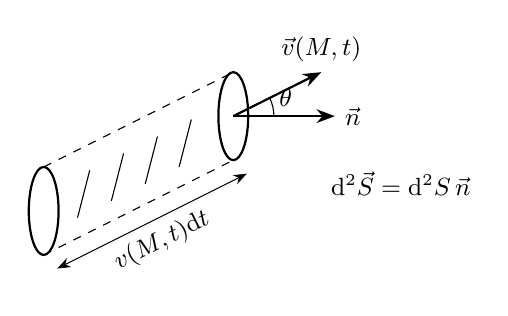
\begin{tikzpicture}[scale=.86]
\draw[edge] (0,0) ellipse (.22 and .65);
\draw[edge] (2.8,1.4) ellipse (.22 and .65);
\draw[dashed] (0,.65)--(2.8,2.05);\draw[dashed] (0,-.65)--(2.8,.75);
\foreach \x in {.5,1,1.5,2}{\draw[thin] (\x,.5*\x-.35)--(\x+.18,.5*\x+.35);}
\draw[flow] (2.8,1.4)--(4.1,2.05) node[above]{$\vv(M,t)$};
\draw[flow] (2.8,1.4)--(4.3,1.4) node[right]{$\vec n$};
\draw (3.4,1.4) arc (0:26.565:.6) node[right]{$\theta$};
\draw[<->] (.2,-.85)--(3,.55) node[midway,below,sloped]{$v(M,t)\dd t$};
\node[right] at (4.1,.4){$\dd^2\vec S=\dd^2S\,\vec n$};
\end{tikzpicture}
\end{center}
La grandeur $\dd^3m$ désigne la masse de fluide qui traverse $\dd^2S$ pendant $\dd t$.
\begin{align*}
\dd^3m&=\mu(M,t)(\dd^2S\,\dd h),\qquad \dd h=v(M,t)\dd t\cos\theta,\\
\dd^3m&=\mu(M,t)\dd t\,\dd^2S\,v(M,t)\cos\theta\\
&=\dd t\,\mu(M,t)\vv(M,t)\cdot\dd^2S\,\vec n,\\
\dd^3m&=\dd t\bigl(\mu(M,t)\vv(M,t)\bigr)\cdot\dd^2S\,\vec n.
\end{align*}
\begin{cadre}
\textbf{Vecteur densité de courant de masse}
\[\JJ(M,t)=\mu(M,t)\vv(M,t).\]
\end{cadre}
\rem
\begin{itemize}\item $\JJ(M,t)$ dépend de $M$ et de $t$.\item Unité : $\mathrm{kg\,s^{-1}\,m^{-2}}$.\end{itemize}
\subsection{Débit massique}
\begin{center}\surface{\Sigma}{1}\qquad $\Sigma$ est une surface quelconque orientée par $\vec n$.\end{center}
\begin{cadre}
On note $D_m$ le \textbf{débit massique} à travers une surface $\Sigma$ orientée.

Il correspond à la masse de fluide qui traverse la surface par unité de temps, comptée positivement dans le sens du vecteur $\dd^2\vec S$ et négativement sinon.\\
Unité : $\mathrm{kg\,s^{-1}}$
\end{cadre}

\begin{cadre}
\[D_m=\iint_\Sigma\JJ(M,t)\cdot\dd^2\vec S.\]
$D_m$ est le flux de $\JJ$ à travers $\Sigma$ orientée.
\end{cadre}
\newpage
% Source : pages 10-12.
\subsection{Équation globale de conservation de la masse}
\underline{Rappel :}
\begin{itemize}
\item Un système ouvert échange de la matière avec l'extérieur.
\item Un système fermé n’échange pas de matière avec l'extérieur.
\end{itemize}
\begin{center}
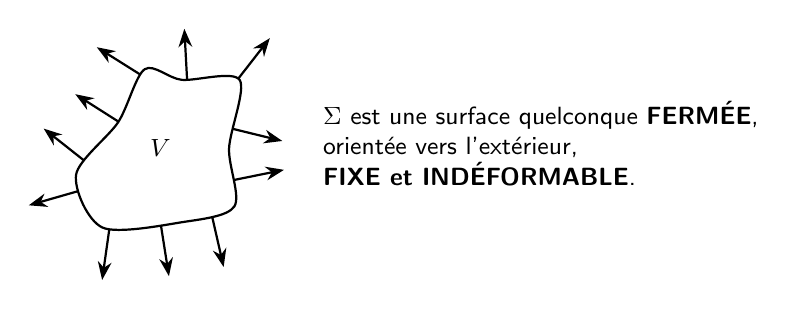
\begin{tikzpicture}[scale=.67]
\draw[edge,postaction={decorate},decoration={markings,
 mark=between positions .03 and .97 step .094 with{\draw[flow] (0,0)--(0,.65);}}]
 plot[smooth cycle] coordinates {(0,0)(-.5,1)(.3,2)(.8,3)(1.5,2.8)(2.6,2.8)(2.4,1.5)(2.5,.4)(1.5,.1)};
\node at (1.1,1.5){$V$};
\node[right,align=left] at (4,1.6){$\Sigma$ est une surface quelconque \textbf{FERMÉE},\\orientée vers l'extérieur,\\ \textbf{FIXE et INDÉFORMABLE}.};
\end{tikzpicture}
\end{center}
On effectue un bilan de masse sur le système ouvert délimité par $\Sigma$, entre $t$ et $t+\dd t$.

D'une part, la masse contenue dans $\Sigma$ s’écrit :
\[
M(t)=\iiint_V\mu(M,t)\dd^3\tau,
\qquad
\frac{\dd M}{\dd t}=\frac{\dd}{\dd t}\iiint_V\mu(M,t)\dd^3\tau
=\iiint_V\pd{\mu}{t}\dd^3\tau.
\]
\textit{La surface étant fixe et indéformable, le domaine d'intégration $V$ est constant.}

D'autre part,
\[
\frac{\dd M}{\dd t}=-D_m\text{ à travers }\Sigma
=-\oiint_\Sigma\JJ(M,t)\cdot\dd^2\vec S.
\]
\textit{Le signe $-$ vient de l’orientation de la surface vers l'extérieur.}

Par \underline{conservation de la masse} :
\[\iiint_V\pd{\mu}{t}\dd^3\tau=-\oiint_\Sigma\JJ(M,t)\cdot\dd^2\vec S.\]
D'où l'équation globale de la conservation de la masse :
\begin{cadre}\[\iiint_V\pd{\mu}{t}\dd^3\tau+\oiint_\Sigma\JJ(M,t)\cdot\dd^2\vec S=0.\]\end{cadre}
\subsection{Équation locale de conservation de la masse}
On applique le théorème de Green-Ostrogradski :
\[\oiint_\Sigma\JJ\cdot\dd^2\vec S=\iiint_V\ddiv\JJ\,\dd^3\tau.\]
Donc
\[\iiint_V\pd{\mu}{t}\dd^3\tau+\iiint_V\ddiv\JJ\,\dd^3\tau=0.\]
\begin{cadre}\[\iiint_V\left(\pd{\mu}{t}+\ddiv\JJ\right)\dd^3\tau=0.\]\end{cadre}
Comme la relation est vraie $\forall\Sigma$, donc $\forall V$,
\[\pd{\mu}{t}+\ddiv\JJ=0,\qquad\text{rappel : }\JJ=\mu(M,t)\vv(M,t).\]
\textbf{L’équation locale de conservation de la masse est appelée équation de continuité.}
\begin{cadre}[etoiles={*****}]\[\pd{\mu}{t}+\ddiv\bigl(\mu(M,t)\vv(M,t)\bigr)=0.\]\end{cadre}
\newpage
% Source : pages 13-15.
\section{Écoulement stationnaire}
\underline{Rappel : définition}
\begin{itemize}\item Tous les champs eulériens qui caractérisent l'écoulement ne dépendent pas du temps.\end{itemize}
\subsection{Propriétés du vecteur densité de courant de masse}
En écoulement stationnaire, $\pd{\mu}{t}=0$, donc
\begin{cadre}\[\ddiv\JJ=0.\]\end{cadre}
Dans un écoulement stationnaire, le vecteur densité de courant de masse est un flux conservatif.

Le flux de $\JJ$ à travers n'importe quelle surface fermée est nul.
\subsection{Conséquence sur le débit massique}
\begin{center}\tube{1}\end{center}
\[
\oiint_\Sigma\JJ\cdot\dd^2\vec S=0
=\iint_{S_1}\JJ\cdot\dd^2\vec S+\iint_{S_2}\JJ\cdot\dd^2\vec S
+\underbrace{\iint_{S_L}\JJ\cdot\dd^2\vec S}_{=0}.
\]
Donc
\[\iint_{S_1}\JJ\cdot\dd^2\vec S+\iint_{S_2}\JJ\cdot\dd^2\vec S=0.\]
\begin{cadre}\[D_{m\,\text{entrant}}=D_{m\,\text{sortant}}.\]\end{cadre}
Dans un écoulement stationnaire, le débit massique est conservé à travers tout tube du champ des vitesses.

\underline{Exemple}
\begin{center}
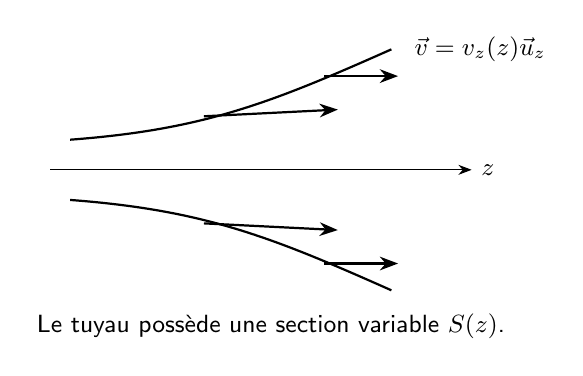
\begin{tikzpicture}[scale=.85]
\draw[->] (-.3,0)--(6,0) node[right]{$z$};
\draw[edge] (0,.45)..controls (2,.6) and (3,1)..(4.8,1.8);
\draw[edge] (0,-.45)..controls (2,-.6) and (3,-1)..(4.8,-1.8);
\draw[flow] (2,.8)--(4,.9);\draw[flow] (3.8,1.4)--(4.9,1.4);
\draw[flow] (2,-.8)--(4,-.9);\draw[flow] (3.8,-1.4)--(4.9,-1.4);
\node[right] at (5,1.8){$\vv=v_z(z)\vec u_z$};
\node[below] at (3,-2){Le tuyau possède une section variable $S(z)$.};
\end{tikzpicture}
\end{center}
\[D_m=\mu(z)S(z)v(z)=\mathrm{cste}.\]
\newpage
% Source : pages 15-17.
\section{Écoulement incompressible}
\subsection{Débit volumique}
\begin{center}\surface{S}{0}\qquad $S$ est une surface fixe orientée.\end{center}
Le \textbf{débit volumique} est le volume de fluide traversant cette surface par unité de temps, compté positivement dans le sens de $\vec n$ et négativement sinon.

Unité : $\mathrm{m^3\,s^{-1}}$ ; dépend de la surface $S$ et du temps $t$.
\subsection{Définition}
Les particules de fluide ont un volume constant lors de l'écoulement.
\[
\left.\begin{array}{l}
\text{Particule}\xrightarrow{\text{fermée}}\dd^3m=\mathrm{cste}\\[8pt]
\text{Si }\dd^3\tau=\mathrm{cste}
\end{array}\right\}\quad
\boxed{\mu(M,t)=\mathrm{cste}\text{ sur la trajectoire}}.
\]
La définition mathématique s’exprime à l’aide de la dérivée particulaire :
\begin{cadre}\[\Dt{\mu}=0.\]\end{cadre}
\underline{Remarques}
\begin{enumerate}[label=\arabic*),leftmargin=7mm]
\item Le caractère incompressible est indépendant du référentiel d'étude.
\item L'écoulement d'un fluide incompressible est toujours incompressible ($\mu=\mathrm{cste}$, pour les liquides).
 \begin{itemize}
\item Un fluide incompressible est une condition plus forte qu'un écoulement incompressible.
\item Un écoulement de gaz peut être supposé incompressible si la vitesse moyenne de l'écoulement est très petite devant la \underline{vitesse du son} (propagation des ondes de pression).\par Ce résultat est démontré en exercice.
\end{itemize}
\end{enumerate}

\newpage
% Source : pages 18-20.
\subsection{Propriété du champ des vitesses}
\[
\pd{\mu}{t}+\underbrace{\ddiv(\mu\vv)}_{=\mu\ddiv(\vv)+\grad\mu\cdot\vv}=0.
\]
\[
\left(\pd{\mu}{t}+\vv\cdot\grad\mu\right)+\mu\ddiv(\vv)=0,
\qquad\Dt{\mu}+\mu\ddiv(\vv)=0.
\]
Donc
\begin{cadre}\[\ddiv(\vv)=-\frac1\mu\Dt{\mu}.\]\end{cadre}
L’écoulement est donc incompressible si et seulement si $\ddiv\vv=0$.

Pour un écoulement incompressible, le champ des vitesses est un flux conservatif.

\underline{Conséquences}
\begin{itemize}\item À $t$ fixé, le flux de $\vv$ à travers n'importe quelle surface fermée est nul.\end{itemize}
\begin{center}\tube{0}\end{center}
\[D_{v1\,\text{entrant}}=D_{v2\,\text{sortant}}.\]
Pour un écoulement incompressible, il y a conservation du débit volumique à travers tout tube du champ des vitesses.
\begin{itemize}\item On considère deux surfaces élémentaires $S_1$ et $S_2$.\end{itemize}
\[v_1\dd S_1=v_2\dd S_2\quad\longrightarrow\quad\dd S_1>\dd S_2\ \Longleftrightarrow\ v_1<v_2.\]
Pour un écoulement incompressible, quand les lignes de champ des vitesses se rapprochent, la norme $\|\vv\|$ augmente.

Si les lignes de champ des vitesses s'éloignent, la norme $\|\vv\|$ diminue.
\newpage
% Source : pages 20-22.
\section{Vecteur tourbillon - Dilatation d'une particule}
\subsection{Problématique mathématique}
Pour un solide étudié dans le référentiel $\mathcal R$, on dispose de la relation suivante :
\[\vv_{\mathcal R}(M)=\vv_{\mathcal R}(N)+\OO_{S/\mathcal R}\wedge\overrightarrow{NM}.\]
Quelle relation peut-on établir pour un fluide ?

Étant donné $\vv(\OM,t)$, on cherche à exprimer $\vv(\OM+\dd\OM,t)$.
\begin{itemize}\item On utilise un développement de Taylor pour une fonction à \underline{quatre variables}.\end{itemize}
On admet la décomposition suivante :
\begin{cadre}
\[\vv(\OM+\dd\OM,t)=\vv(\OM,t)+\OO\wedge\dd\OM+\vec d,\]
\[\text{avec}\quad\OO=\frac12\rot\vv,\qquad\vec d=[D]\dd\OM.\]
La matrice $[D]\in\mathcal M_3$ s’écrit :
\[
[D]=\begin{pmatrix}a_1&0&0\\0&a_2&0\\0&0&a_3\end{pmatrix}
+\begin{pmatrix}0&g_3&g_2\\g_3&0&g_1\\g_2&g_1&0\end{pmatrix},
\qquad\operatorname{tr}(D)=\ddiv(\vv).
\]
\[
\left\{\begin{aligned}a_1&=\pd{v_x}{x}\\[4pt]a_2&=\pd{v_y}{y}\\[4pt]a_3&=\pd{v_z}{z}\end{aligned}\right.
\qquad
\left\{\begin{aligned}g_1&=\frac12\left(\pd{v_y}{z}+\pd{v_z}{y}\right)\\[4pt]g_2&=\frac12\left(\pd{v_z}{x}+\pd{v_x}{z}\right)\\[4pt]g_3&=\frac12\left(\pd{v_x}{y}+\pd{v_y}{x}\right).\end{aligned}\right.
\]
\end{cadre}
Le terme $\OO\wedge\dd\OM$ décrit une rotation comme celle d’un solide.

On définit le \textbf{vecteur tourbillon} par $\OO=\frac12\rot(\vv)$.
\begin{itemize}\item Il représente le vecteur de rotation locale.\end{itemize}
Le vecteur $\vec d$ correspond à la déformation.
\begin{itemize}
\item Cette déformation s’accompagne-t-elle d’une variation de volume ?
\item Si $\ddiv(\vv)=0$, il n’y a pas de variation de volume.
\item Si $\ddiv(\vv)\ne0$, le volume varie.
\end{itemize}
\begin{cadre}\[\ddiv\vv=-\frac1\mu\Dt{\mu}.\]\end{cadre}
\begin{cadre}\[\ddiv\vv=\frac1{\dd^3\tau}\Dt{(\dd^3\tau)},\qquad\text{avec}\quad\mu=\frac{\dd^3m}{\dd^3\tau}.\]\end{cadre}
\textit{Il n’y a pas de signe moins dans cette expression, car la différentiation produit un second signe moins.}
\newpage
% Source : pages 22-24.
\subsection{Quelques exemples}
\textbf{a)}\quad $\displaystyle\vv(M,t)=\begin{pmatrix}a_1x\\b_1y\end{pmatrix},\qquad a_1>0,\quad b_1<0,\quad a_1+b_1\ne0.$

Cet écoulement est \underline{plan et stationnaire}.
\[\ddiv\vv=\pd{v_x}{x}+\pd{v_y}{y}=a_1+b_1\ne0.\]
\[
\rot\vv=\begin{pmatrix}\pd{}{x}\\[3pt]\pd{}{y}\\[3pt]\pd{}{z}\end{pmatrix}
\wedge\begin{pmatrix}a_1x\\b_1y\\0\end{pmatrix}=\vec0.
\]
\begin{cadre}\[\rot\vv=\vec0.\]\end{cadre}
\begin{center}\deformation{1}\end{center}
\(\rightarrow\) La particule a subi une déformation avec variation de volume.
\begin{align*}
V(t)&=L^3,\\
V(t+\dd t)&=L(L+a_1L\dd t)(L+b_1L\dd t)\\
&\simeq L^3\bigl(1+(a_1+b_1)\dd t\bigr).
\end{align*}
\textit{On effectue un développement limité à l'ordre 1.}
\[\frac{V(t+\dd t)-V(t)}{V(t)}=(a_1+b_1)\dd t=\ddiv\vv.\]

\textbf{La particule se déforme sans rotation locale, avec dilatation.}
\newpage
% Source : pages 24-25.
\textbf{b)}\quad $\displaystyle\vv(M,t)=\begin{pmatrix}a_2y\\a_2x\end{pmatrix},\qquad a_2>0.$

Cet écoulement est plan et stationnaire.
\[\ddiv\vv=\pd{v_x}{x}+\pd{v_y}{y}=0\quad\longrightarrow\quad\text{il n’y a pas de dilatation}.\]
\[
\rot\vv=\begin{pmatrix}\pd{}{x}\\[3pt]\pd{}{y}\\[3pt]\pd{}{z}\end{pmatrix}
\wedge\begin{pmatrix}a_2y\\a_2x\\0\end{pmatrix}=\vec0.
\]
\begin{center}\deformation{2}\end{center}
\[\ddiv\vv=\frac1{\dd^3V}\Dt{(\dd^3V)}.\]
\textbf{La particule se déforme sans rotation locale et sans dilatation.}
\par\vspace{9mm}\par
\textbf{c)}\quad $\displaystyle\vv(M,t)=\begin{pmatrix}-a_3y\\a_3x\\0\end{pmatrix},\qquad a_3>0.$

Cet écoulement est plan et stationnaire.
\[\ddiv\vv=0.\]
\[
\rot\vv=\begin{pmatrix}\pd{}{x}\\[3pt]\pd{}{y}\\[3pt]\pd{}{z}\end{pmatrix}
\wedge\begin{pmatrix}-a_3y\\a_3x\\0\end{pmatrix}=\begin{pmatrix}0\\0\\2a_3\end{pmatrix}.
\]
\[\rot\vv=2a_3\vec u_z\quad\longrightarrow\quad\text{il y a une rotation locale}.\]
\newpage
% Source : pages 25-28.
\begin{center}\deformation{3}\end{center}
\[
L\dd\theta=a_3L\dd t,\qquad \dot\theta=a_3,
\qquad\OO=\dot\theta\vec u_z=a_3\vec u_z=\frac12\rot\vv.
\]
\textbf{La particule tourne en bloc} et, dans ce cas, ne se déforme pas.
\subsection{Généralisation}
Le mouvement d'une particule de fluide est caractérisé, d'une part, par une rotation et une translation localement.

Cette rotation locale est caractérisée par le vecteur tourbillon $\OO=\frac12\rot\vv$.
\[\OO(M,t)\quad\longrightarrow\quad\OO\text{ dépend de chaque point du fluide}.\]
\rem Le vecteur $\rot\vv$ est appelé vecteur vorticité.

D'autre part, le mouvement est caractérisé par une déformation, avec ou sans dilatation.
\subsection{Cas de l'écoulement irrotationnel}
\[\text{Écoulement irrotationnel}\ \Longleftrightarrow\ \rot\vv=\vec0\ \Longleftrightarrow\ \OO=\vec0.\]
Dans le cas contraire, l’écoulement est dit rotationnel ou tourbillonnaire.

\underline{Remarques}
\begin{itemize}
\item Dans un écoulement, le caractère tourbillonnaire est un caractère local.
\item Le caractère tourbillonnaire \underline{dépend du référentiel}.
\item Il n'est pas possible (a priori) de prévoir le caractère tourbillonnaire d'un écoulement sans calcul.
\end{itemize}
\textbf{Attention :} avoir des lignes de courant circulaires n’est pas équivalent à être un écoulement tourbillonnaire.

\textbf{Attention :} avoir des lignes de courant parallèles n’est pas équivalent à être un écoulement non tourbillonnaire.
\newpage
% Source : pages 28-29. Les pages 30 et 31 du PDF source sont vides.
\(\rightarrow\) Dans un écoulement irrotationnel,
\[\rot\vv=\vec0.\]
\begin{cadre}[etoiles={***}]
\[\exists\phi(M,t)\text{, potentiel des vitesses, tel que }\vv=\grad\phi.\]
On peut se reporter au polycopié de mathématiques.
\end{cadre}
Un écoulement irrotationnel est aussi appelé écoulement potentiel.
\subsection{Cas de l'écoulement irrotationnel et incompressible}
\[\ddiv(\vv)=0\quad\text{donc}\quad\ddiv(\grad\phi)=0.\]
Alors
\begin{cadre}[etoiles={*****}]\[\Delta\phi=0.\]\begin{center}\textbf{Équation de Laplace}\end{center}\end{cadre}
\underline{Remarques}
\begin{itemize}
\item On rencontre des relations analogues dans l’étude de la diffusion, en électricité et dans d’autres domaines.
\item L'équation de Laplace est \underline{linéaire} ; le théorème de superposition est donc valable.
\item La solution est \underline{unique} lorsque les conditions aux limites sont fixées.
\end{itemize}
\end{document}